\documentclass{article}

\pdfoutput=1

\usepackage[utf8]{inputenc}
\usepackage[T1]{fontenc}
\usepackage[english]{babel}
\usepackage{amsmath}
\usepackage{mathtools}
\usepackage{lmodern}
\usepackage{units}
\usepackage{siunitx}
\usepackage{icomma}
\usepackage{graphicx}
\usepackage{caption}
\usepackage{subcaption}
\usepackage{color}
\newcommand{\N}{\ensuremath{\mathbbm{N}}}
\newcommand{\Z}{\ensuremath{\mathbbm{Z}}}
\newcommand{\Q}{\ensuremath{\mathbbm{Q}}}
\newcommand{\R}{\ensuremath{\mathbbm{R}}}
\newcommand{\C}{\ensuremath{\mathbbm{C}}}
\newcommand{\rd}{\ensuremath{\mathrm{d}}}
\newcommand{\id}{\ensuremath{\,\rd}}
\usepackage{hyperref}
%\usepackage{a4wide} % puts the page numbering further down the page.
\usepackage{pdfpages}
\usepackage{epstopdf}
\DeclareMathOperator{\sgn}{sgn}
\DeclareGraphicsExtensions{.eps}

\title{Home Assigment Week 3}
\author{Marcus Malmquist, marmalm, 941022}
\date{\today}

\begin{document}
\maketitle

\section{Task 1}\label{sec:1}
The circuit in Figure~\ref{fig:circ} will be used to design a $\SI{3}{\deci\bel}$ attenuator.
\begin{figure}
  \centering
  \noindent\makebox[\textwidth]{\scalebox{0.9}{\input{circuit.pdf_t}}}
  \caption{The figure depicts a circuit that will be used as $\SI{3}{\deci\bel}$ attenuator.}
  \label{fig:circ}
\end{figure}

\subsection{a}\label{sec:1a}
Looking at Figure~\label{fig:smith} it can be concluded that if the transmission line is lossless and the circuit must be matched to the input impedance, this circuit can not function as a $\SI{3}{\deci\bel}$ attenuator. Assuming reflections will not be a problem for this system, the potential at the output of the circuit can be acquired using voltage division (\ref{eq:voltdiv}).
\begin{figure}
  \centering
  \noindent\makebox[\textwidth]{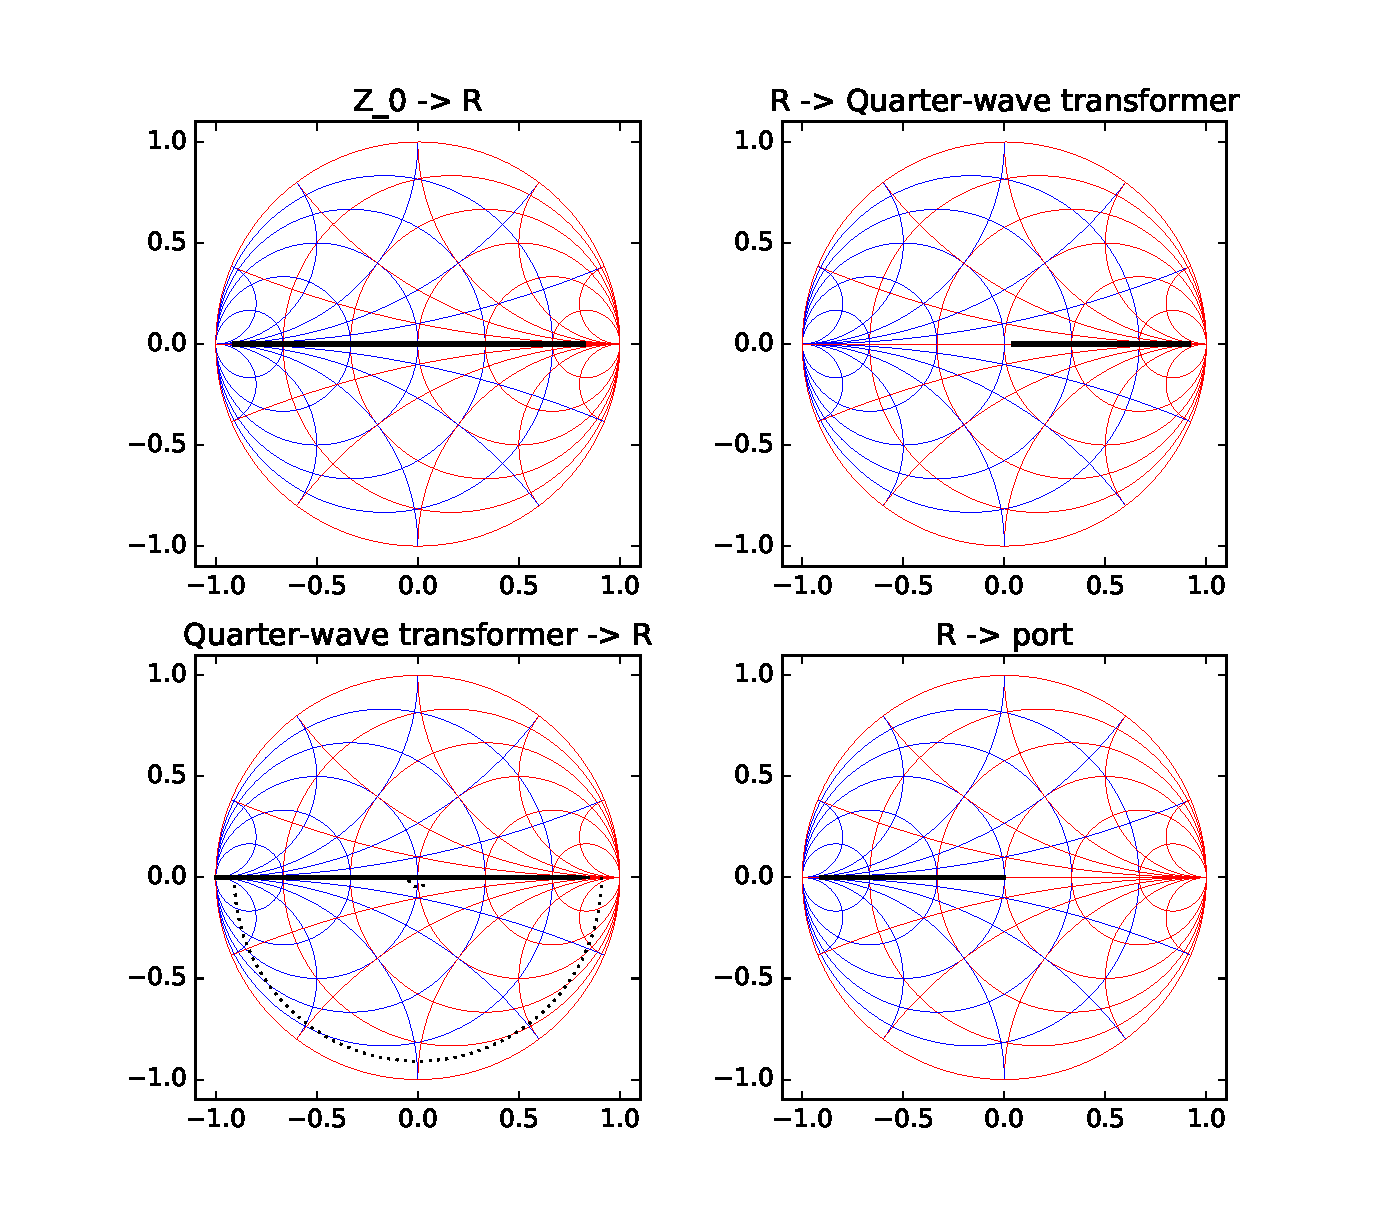
\includegraphics{Smith.pdf}}
  \caption{The figure depicts $\Gamma$/$Z_\text{in}$ for values of $R$ ranging from $\SI{5}{\ohm}$ to $\SI{1}{\kilo\ohm}$ at each interface between neighbouring components in the circuid show in Figure~\ref{fig:circ}. A characteristic impedance of $\SI{50}{\ohm}$ was used and the Smith chart on the lower right-hand side is $Z_\text{in}$ at the port.}
  \label{fig:smith}
\end{figure}
\begin{equation}
  V_\text{out} = V_\text{in}\dfrac{Z_c}{Z_\text{in}}=V_\text{in}\dfrac{Z_c}{R+\frac{Z_c^2}{R+Z_c}}
  \label{eq:voltdiv}
\end{equation}
Since we require that the circuit is a $\SI{3}{\deci\bel}$ attenuator we end up with (\ref{eq:R}).
\begin{equation}
  R=\dfrac{\sqrt{2}-1+\sqrt{2\sqrt{2}-1}}{2}Z_c\approx 0.88Z_c
  \label{eq:R}
\end{equation}
The Smith chart for the circuit using the value of $R$ from (\ref{eq:R}) can be seen in Figure~\ref{fig:smithr}.
\begin{figure}
  \centering
  \noindent\makebox[\textwidth]{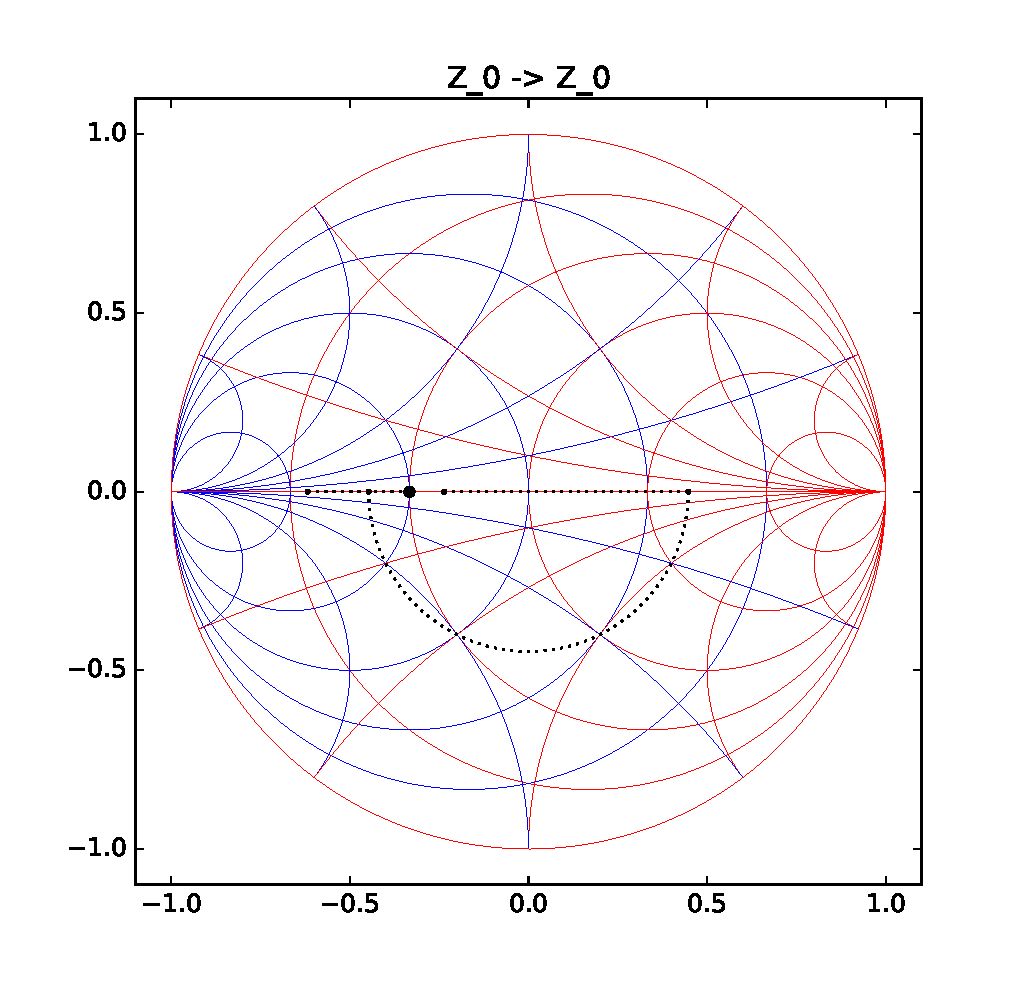
\includegraphics{SmithR.pdf}}
  \caption{The figure depicts $\Gamma$/$Z_\text{in}$ for the value of $R$ from (\ref{eq:R}) at each interface between neighbouring components in the circuid show in Figure~\ref{fig:circ}. The chart is independent of characteristic impedance.}
  \label{fig:smithr}
\end{figure}
\subsection{b}\label{sec:1b}
The return input reflection is $\Gamma=-0.17$ and return loss is $\SI{15.3}{\deci\bel}$.

\section{Task 2}\label{sec:2}
The solution to the matching system in Figure~\ref{fig:match} can be seen in Figure~\ref{fig:smith_match}. In order to get a broaded wideband the solution that had the shortest components was used. The resulting values at $\SI{1800}{\mega\hertz}$ are $d=0.258\lambda=\SI{42.9}{\milli\metre}$ and $l=0.171\lambda=\SI{28.4}{\milli\metre}$.

As I do not have access to \textit{ADS} and is therefor unable to calculate the dimensions of the microstrip circuit.
\begin{figure}
  \centering
  \begin{subfigure}[b]{\textwidth}
    \centering
    \noindent\makebox[\textwidth]{\scalebox{0.9}{\input{match.pdf_t}}}
    \subcaption{The equivalent circuit that will be used to match an inverted-F antenna.}
    \label{fig:match}
  \end{subfigure}\\
  \begin{subfigure}[b]{\textwidth}
    \centering
    \noindent\makebox[\textwidth]{\scalebox{0.9}{\input{match_strip.pdf_t}}}
    \subcaption{An example of a microstrip realization of the matching circuit for an inverted-F antenna.}
    \label{fig:match_strip}
  \end{subfigure}
  \caption{The figure depicts the matching curcuit for the inverted-F antenna.}
  \label{fig:match}
\end{figure}
\begin{figure}
  \centering
  \noindent\makebox[\textwidth]{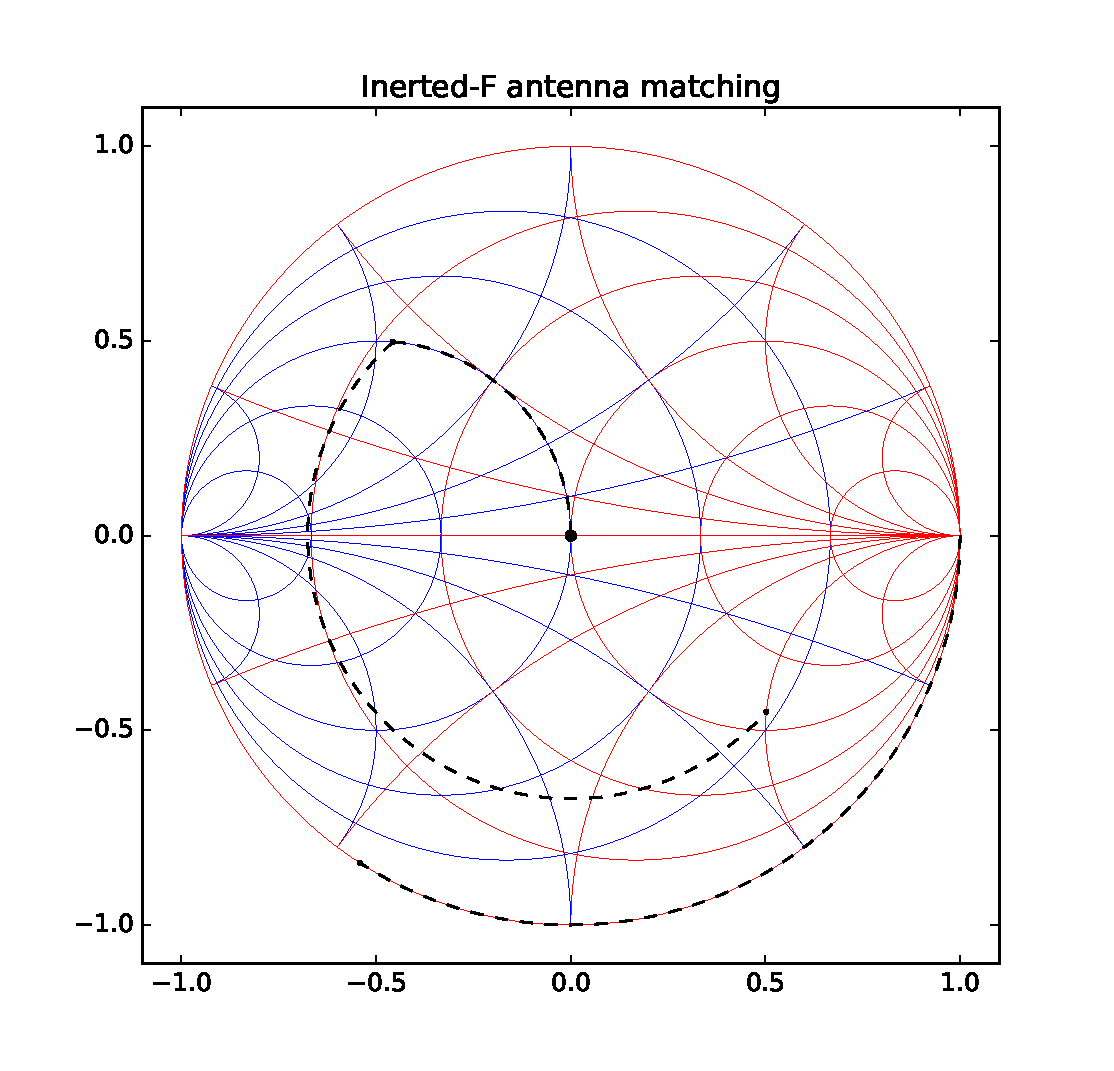
\includegraphics{invert_f_match.pdf}}
  \caption{The figure depicts the Smith chart for matching an inverted-F antenna with an antenna impedance of $\SI{60-j100}{\ohm}$ to a $\SI{50}{\ohm}$ line at $\SI{1800}{\mega\hertz}$.}
  \label{fig:smith_match}
\end{figure}

\end{document}